 % !TEX program = lualatex
\documentclass[xcolor={x11names, table},compress]{beamer}

\usepackage{xcolor}
\usepackage{fontspec}
\usepackage{pgfplots}
\usepackage{tikz}
\usepackage{amsmath, amssymb, amsfonts}
\usepackage{bm}
\usepackage{eso-pic}
\usepackage{graphicx}

\pgfplotsset{compat=1.15}
\usetikzlibrary{positioning, shapes, calc, arrows}
\hypersetup{pdfstartview={Fit}}

%% Beamer Layout %%%%%%%%%%%%%%%%%%%%%%%%%%%%%%%%%%
\useinnertheme{default}
\usefonttheme{serif}
\usepackage{palatino}
\usepackage[T1]{fontenc}
\usepackage[default]{lato}

\setbeamerfont{frametitle}{}

\definecolor{BHKpresentationDark}{RGB}{114,133,176}
\definecolor{BHKpresentationDarkGrey}{RGB}{103,116,128}
\definecolor{BHKblue}{RGB}{51,105,153}

\setbeamerfont{title like}{shape=\scshape}
\setbeamercolor*{frametitle}{fg=BHKpresentationDark} 
\setbeamercolor*{lower separation line head}{bg=BHKblue} 
\setbeamercolor*{normal text}{fg=BHKpresentationDarkGrey,bg=white} 
\setbeamercolor*{alerted text}{fg=BHKblue} 
\setbeamercolor*{example text}{fg=black} 
\setbeamercolor*{item}{fg=BHKpresentationDark,bg=gray} 
\setbeamercolor{enumerate item}{fg=BHKpresentationDark}
\setbeamercolor*{structure}{fg=black} 
\setbeamercolor*{palette tertiary}{fg=black,bg=black!10} 
\setbeamercolor*{palette quaternary}{fg=black,bg=black!10} 
\setbeamercovered{transparent}

\setbeamertemplate{navigation symbols}{}
\setbeamertemplate{footline}{%
    \begin{beamercolorbox}[wd=\paperwidth]{footlinecolor}
        
\includegraphics[width=\textwidth]{bar_footline.pdf}
    \end{beamercolorbox}%
}

\setbeamertemplate{frametitle}[default][center]
\setbeamertemplate{caption}[numbered]
\setbeamertemplate{section in toc}[sections numbered]
\setbeamertemplate{subsection in toc}[subsections numbered]

\newcommand{\insertsec}{\thesection.~\insertsection}
\newcommand{\insertsubsec}{\thesection.\thesubsection~\insertsubsection}

%%%% Start of document %%%%%%%%%%

\begin{document}
%%%% title slide %%%%%
{\setbeamertemplate{footline}{} 
    \begin{frame}
    
    \vspace{-1.5cm}
    \hfill\makebox[0.2\paperwidth]{
\includegraphics[width=0.4\textwidth]{logo_wtext}}
    \begin{flushleft}
        \hspace{-1cm}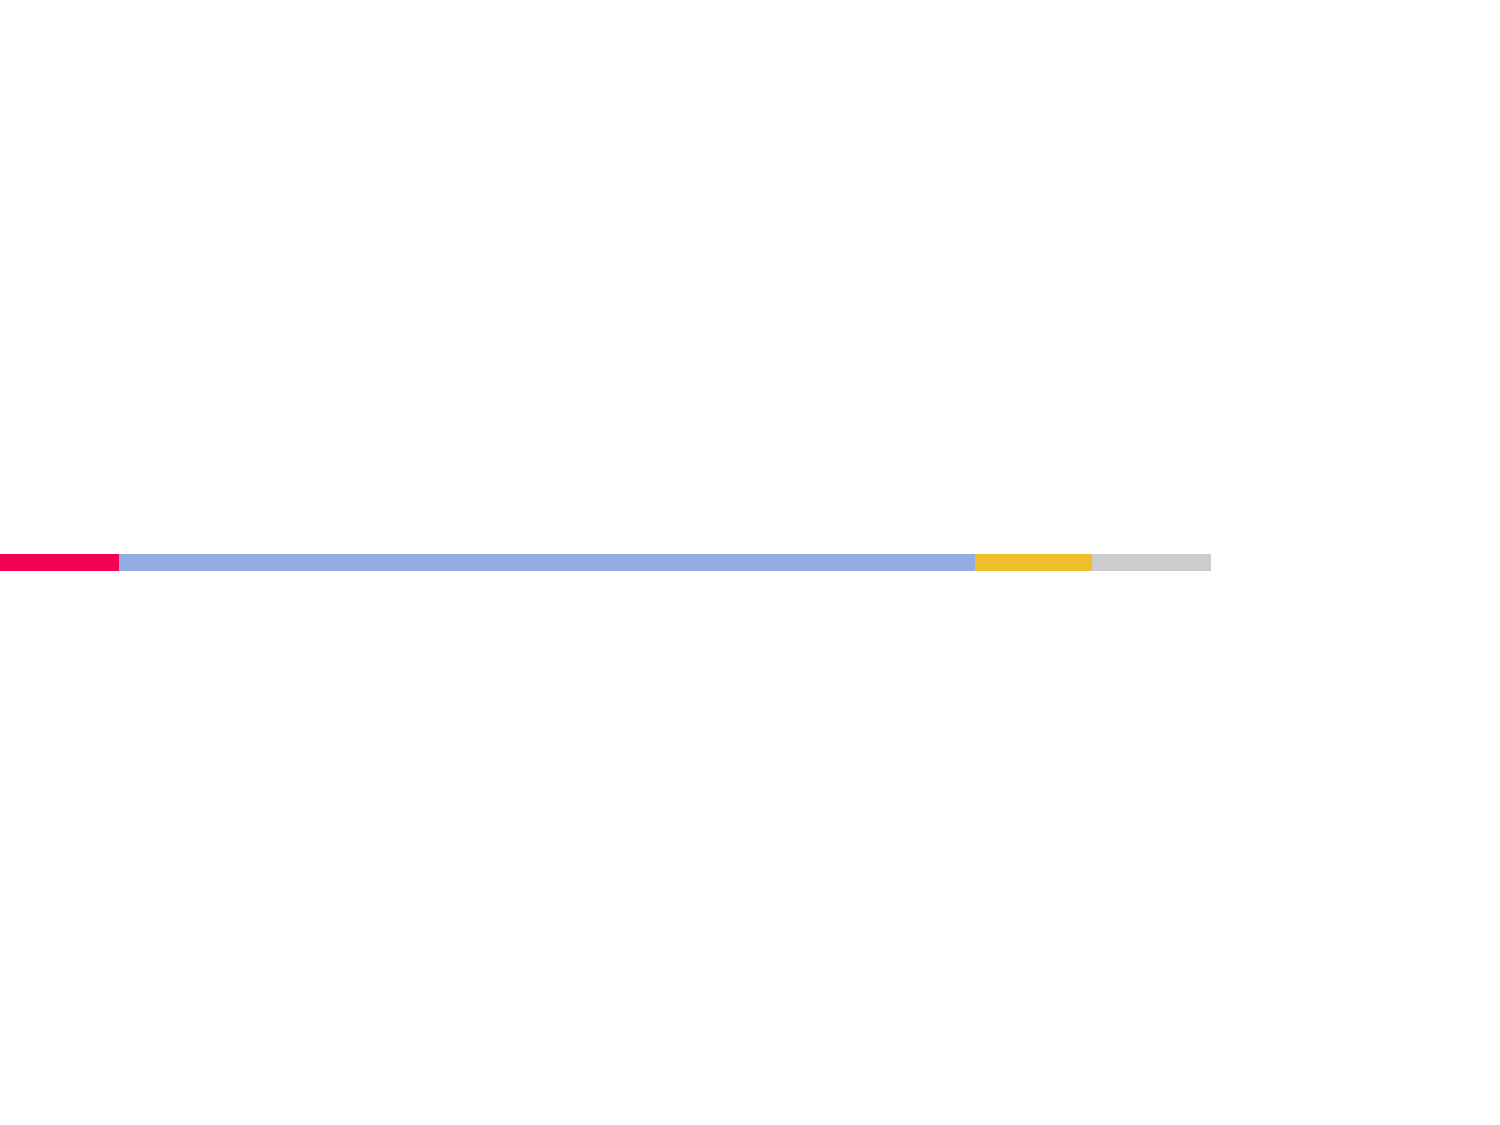
\includegraphics[width=0.8\textwidth, height=0.4em]{title_line.pdf}\hfill
        
        \title{
            \begin{flushleft}{\huge \color{BHKpresentationDark} Convolutional Neural Networks Summary} 
        \end{flushleft}}
        
        % \date{\today}
        \date{$~~$}
        \author[Joan]{\begin{flushleft}\vspace{-1cm} Joan Marcè i Igual\end{flushleft}}
        \titlepage
    \end{flushleft}
\end{frame}
}

\begin{frame}{Table of Contents}
	\tableofcontents
\end{frame}

\section{Introduction}
\begin{frame}{\insertsec}
	Neural Networks are a type of supervised learning. So we have a set of labeled data:
	$$\{(x^{(1)}, y^{(1)}), (x^{(2)}, y^{(2)}), ..., (x^{(m)}, y^{(m)})\}$$
	
	We want to use it to predict new data $\hat{y} = f(x)$
	
	\textbf{Problem}: search the proper $f(x)$
\end{frame}
\section{Neural Networks}
\begin{frame}{\insertsec}
	
\tikzset{
  pics/layer/.style n args = {3}{
    code = {
      \foreach \y in {1,...,#1} {
        \node[draw, circle] (L-#2-\y) at (0,{1.5*(\y - #1/2)}) {${#3}_{#2 \y}$};
      }
    }
  }
}

\begin{tikzpicture}
\def\layers{2/I, 5/H, 5/H, 3/O}

\foreach \x/\name [count=\xi] in \layers  {
  \draw (3*\xi, 0) pic {layer={\x}{\xi}{\name}};
}

\foreach \x/\ignore [count=\xi, remember=\xi as \lastxi, remember=\x as \lastx] in \layers {
  \ifthenelse{\xi > 1}{
    \foreach \ylast in {1,...,\lastx} \foreach \y in {1,...,\x}{
      \draw [-latex] (L-\lastxi-\ylast) -- (L-\xi-\y);
    }
  }{};
}

\end{tikzpicture}


\end{frame}
\subsection{Parameters}
\begin{frame}{\insertsubsec}
    \begin{columns}[t]
        \column{.6\textwidth}
        \begin{itemize}
            \item $l$: Current layer
            \item $w_{i, j}^{[l]}$: Weight from neuron $j$ to $i$ at layer $l$
            \item $b_{i}^{[l]}$: Bias for neuron $i$ at layer $l$
            \item $n^{[l]}$: Neurons for layer $l$
            \item $\bm{W}^{[l]} \in \mathbb{R}^{n^{[l]} \times n^{[l - 1]}}$: Weight matrix
            \item $\bm{b}^{[l]} \in \mathbb{R}^{n^{[l]}}$: Bias
            \item $
            \begin{aligned}[t]
            \bm{a}^{[l]} &= g(\bm{W}^{[l]}\cdot \bm{a}^{[l - 1]} + \bm{b}^{[l]}) \\
            \bm{a}^{[l]} &\in \mathbb{R}^{n^{[l]}}
            \end{aligned}
            $ Activations for layer $l$
            \item $g(x)$: Activation function
        \end{itemize}
        \column{.5\textwidth}
        \centering
        \begin{columns}[t]
    \column{.5\textwidth}
    \centering
    \begin{figure}
        \begin{tikzpicture}
            \begin{axis}[
                width=\textwidth,
                height=.8\textwidth,
                grid=major,
                grid style={dashed, gray!30},
                xtick={-5, 0, 5},
                xticklabels={$-\infty$, $0$, $+\infty$}
                ]
                \addplot[mark=none]{tanh(x)};
            \end{axis}
        \end{tikzpicture}
        \caption{$\tanh(x)$}
    \end{figure}
    \centering
    \column{.5\textwidth}
    \begin{figure}
        \begin{tikzpicture}
            \begin{axis}[
                width=\textwidth,
                height=.8\textwidth,
                grid=major,
                grid style={dashed, gray!30},
                xtick={-5, 0, 5},
                xticklabels={\empty, $0$, \empty}
                ]
                \addplot[mark=none]{max(x, 0)};
            \end{axis}
        \end{tikzpicture}
        \caption{ReLU function}
    \end{figure}
\end{columns}
    \end{columns}
\end{frame}
\begin{frame}
    \begin{columns}
        \column{.6\textwidth}
        \begin{block}{Cost function}
            $$
            J(\bm{W}, \bm{b}, \hat{\bm{y}}, \bm{y}) = \frac{1}{m} \sum_{i=1}^{m} \mathcal{L}(\hat{\bm{y}}^{(i)}, \bm{y}^{(i)})
            $$
        \end{block}
        \begin{block}{Loss function}
            $$
            \mathcal{L}(\hat{\bm{y}}, \bm{y}) = ||\hat{\bm{y}} - \bm{y}||^2
            $$
        \end{block}
        \begin{block}{Parameters update}
            \begin{align*}
            \bm{W} &:= \bm{W} - \alpha*\frac{\partial J}{\partial \bm{W}} \\
            \bm{b} &:= \bm{b} - \alpha*\frac{\partial J}{\partial \bm{b}}
            \end{align*}
        \end{block}
        \column{.4\textwidth}
        To achieve better results at predicting $\hat{\bm{y}}$ we have to minimize the cost function $J(\bm{W}, \bm{b}, \hat{\bm{y}}, \bm{y})$.
    \end{columns}
\end{frame}

\section{Convolutional Neural Networks}
\begin{frame}{\insertsec}
    This type of networks are a bit different because instead of computing the activations by
    multiplying the previous ones with the weight matrix it convolutes the previous activations (denoted by $*$):
    
    \begin{align*}
        \bm{a}^{[l]} &= g(\bm{W}^{[l]}\cdot \bm{a}^{[l - 1]} + \bm{b}^{[l]}) \\
        \text{Becomes:} \\
        \bm{a}^{[l]} &= g(\bm{W}^{[l]} * \bm{a}^{[l-1]} + \bm{b}^{[l]})
    \end{align*}
\end{frame}

\subsection{Convolution Operation}
\begin{frame}{\insertsubsec}
    \begin{align*}
        \left(
        \begin{array}{cccccc}
            10 & \cellcolor{green!20}10 & \cellcolor{green!20}10 & \cellcolor{green!20}0 & 0 & 0 \\
            10 & \cellcolor{green!20}10 & \cellcolor{green!20}10 & \cellcolor{green!20}0 & 0 & 0 \\
            10 & \cellcolor{green!20}10 & \cellcolor{green!20}10 & \cellcolor{green!20}0 & 0 & 0 \\
            10 & 10 & 10 & 0 & 0 & 0 \\
            10 & 10 & 10 & 0 & 0 & 0 \\
            10 & 10 & 10 & 0 & 0 & 0 \\
        \end{array}
        \right)
        *
        \left(
        \begin{array}{ccc}
            1 & 0 & -1 \\
            1 & 0 & -1 \\ 
            1 & 0 & -1 \\
        \end{array}
        \right)
        = 
        \left(
        \begin{array}{cccc}
            0 & \cellcolor{green!20}30 & 30 & 0 \\
            0 & 30 & 30 & 0 \\
            0 & 30 & 30 & 0 \\
            0 & 30 & 30 & 0 \\
        \end{array}
        \right)
    \end{align*}

\end{frame}


\end{document}